\documentclass[letterpaper,10pt,titlepage]{article}

\usepackage{graphicx}

\usepackage{amssymb}
\usepackage{amsmath}
\usepackage{amsthm}

\usepackage{alltt}
\usepackage{float}
\usepackage{color}
\usepackage{verbatim}

\usepackage{geometry}
\geometry{textheight=10in, textwidth=7.5in}

\usepackage{hyperref}

\def\name{Jordan Bayles (baylesj)}

%pull in the necessary preamble matter for pygments output
\input{pygments.tex}

%% The following metadata will show up in the PDF properties
\hypersetup{
  colorlinks = true,
  urlcolor = black,
  pdfauthor = {\name},
  pdfkeywords = {cs311 ``operating systems'' files filesystem I/O},
  pdftitle = {CS 311 Project 3: UNIX Process Control},
  pdfsubject = {CS 311 Project 3},
  pdfpagemode = UseNone
}

\parindent = 0.0 in
\parskip = 0.2 in

\begin{document}
\section{System design}
I laid the program out into three main parts: parser, sorters, and suppressor.
I originally planned on forking all three from one function (and then passing the
run function to utilize through a function prototype) but this proved to be
infeasible so I went with specialized forking functions.

\section{Work log}
\verbatiminput{git_log.txt}

\section{Timing}
Ran on Les Miserable, number of copies of text shown.
\begin{center}
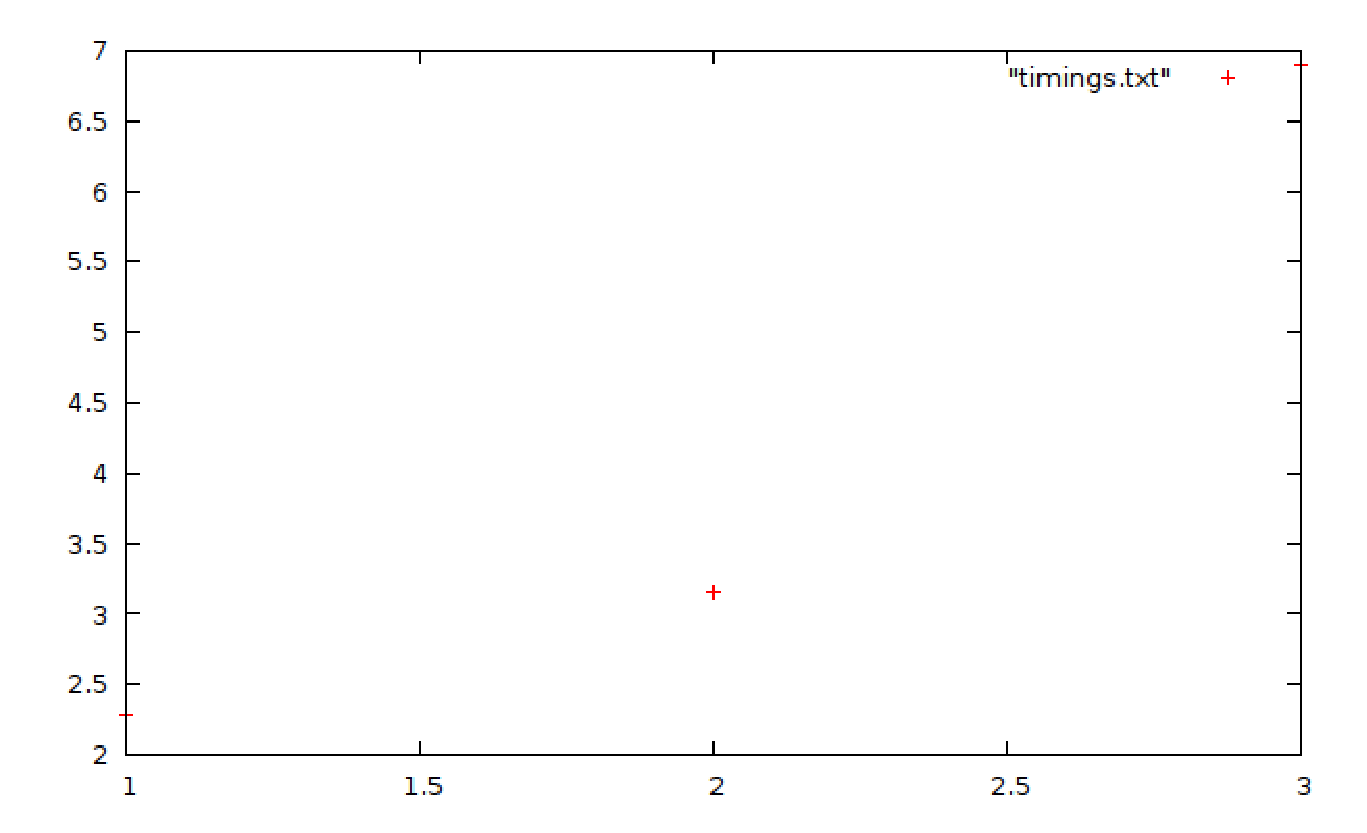
\includegraphics[width=4in]{graph.eps}
\end{center}

\section{Challenges}
Biggest challenge was definitely getting the pipes to behave correctly. I also
struggled with debugging (using gdb) on multiple processes. Even using the
"set follow-fork-mode parent/child" command was still a pain to do.

\section{Output}
\begin{figure}[H]
	\caption{Run times with various file sizes}
	\includegraphics[width=\textwidth]{runtime.eps}
\end{figure}

\section{Questions}
\subsection{Main point of the assignment}
Multiple processes (fork()) and pipes specifically. Probably also some general
system knowledge, fd manipulation, etc.

\subsection{Solution testing}
gdb, valgrind. Mostly testing on files from Project Gutenburg with different numbers
of processes and checking output. Checked on small input files at first to get an
expected output.

\subsection{I learned...}
How to handle pipes correctly and deal with the issues caused by forking off multiple
child processes within a single application.

\end{document}
